%!TEX root = ../../root.tex

We have seen that we can do something when we approach the manifolds \emph{extrinsically}, meaning operating in the $3D$ space where the object lives.
However, such a filter would not be \emph{deformation} invariant, since it will not bend along with the object.

\begin{figure}[H]
    \centering
    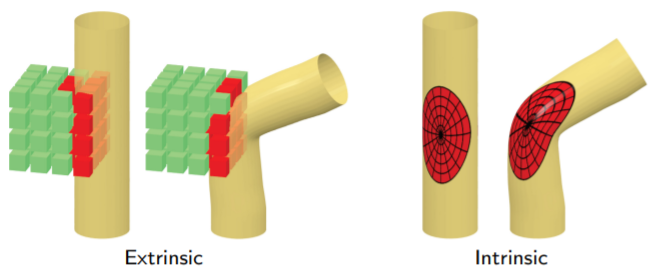
\includegraphics[width=.7\textwidth]{figures/12/12_46.png}
    \caption{Extrinsic vs Intrinsic.}
\end{figure}

We would like for the filters to operate directly on the surface, so that they deform along with the object, and thus obtain deformation invariance \emph{by construction}, since we have defined our convolutional kernel directly on the 
surface, not on the Euclidean domain.

\begin{figure}[H]
    \centering
    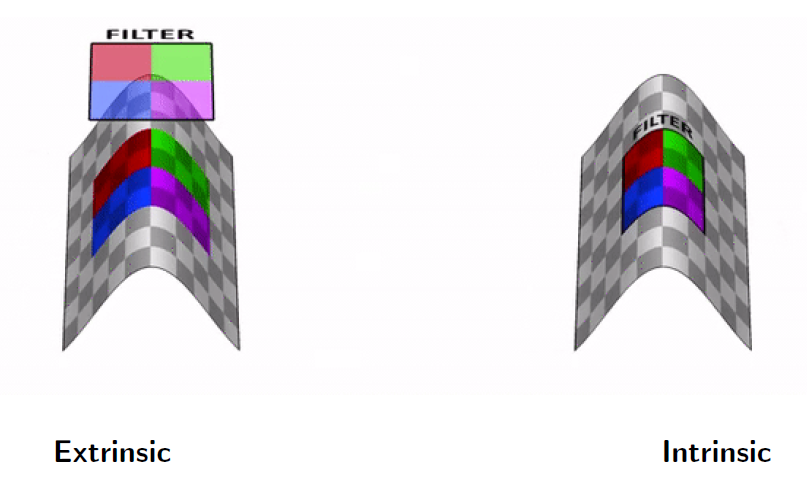
\includegraphics[width=.7\textwidth]{figures/12/intrinsic.png}
    \caption{Extrinsic vs Intrisc.}
\end{figure}

But how to define such a non-Euclidean convolution?

Convolution relies on the grid-like structure of the Euclidean space, in which there is a well-behaved concept of distance and neighborhood. But how would you perform convolution on a graph?
Suppose each node $v$ has a scalar feature $x(v)$, just like each pixel $i, j$ of an image has an intensity $f(i, j)$. In the case of an image we would convolve with a $3 \times 3$ kernel $g$ like so
\begin{equation}
    (g \star f)[i, j] = \sum_{m = 1}^3 \sum_{n = 1}^3 g[m, n] f[i-m, j-n]
\end{equation}
in which we are exploiting the grid-like Euclidean structure to extract a \emph{local patch} of \emph{adjacent} pixels, then considered in a certain order (the indices of the summations) to properly combine them with the filter. But what would be a local patch for a node in a graph? Its immediate neighborhood? But then each node would have a neighborhood of different size, so we could not have weight sharing by using the same filter. Even if this was not already a problem, what would be such ordering for the neighborhood of a node?

Unlike images, there is no canonical ordering of the domain points in graphs and meshes, and the absence of this concept is a critical issue, named \emph{local ambiguity}. In a graph there is no canonical way of visiting the neighbors of a node. In a mesh we have a notion of orientation, and from that we could label the neighbors of a node in a clockwise fashion, but then how would we fix the first node in the cycle, to begin our visit? This would still be ambiguous.
\begin{figure}[H]
    \centering
    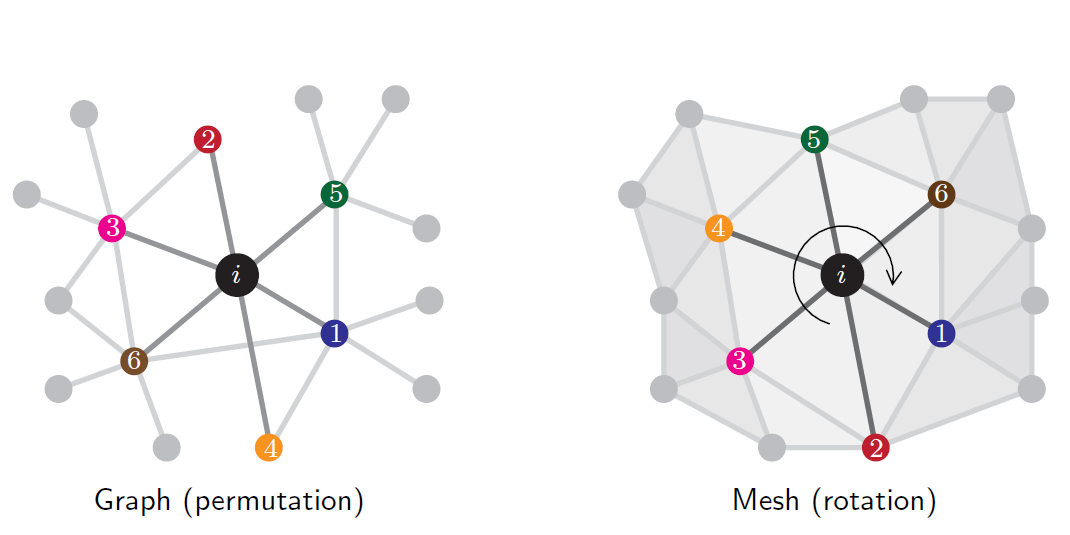
\includegraphics[width=.7\textwidth]{figures/12/local.png}
    \caption{Local ambiguity.}
\end{figure}

\begin{figure}[H]
    \centering
    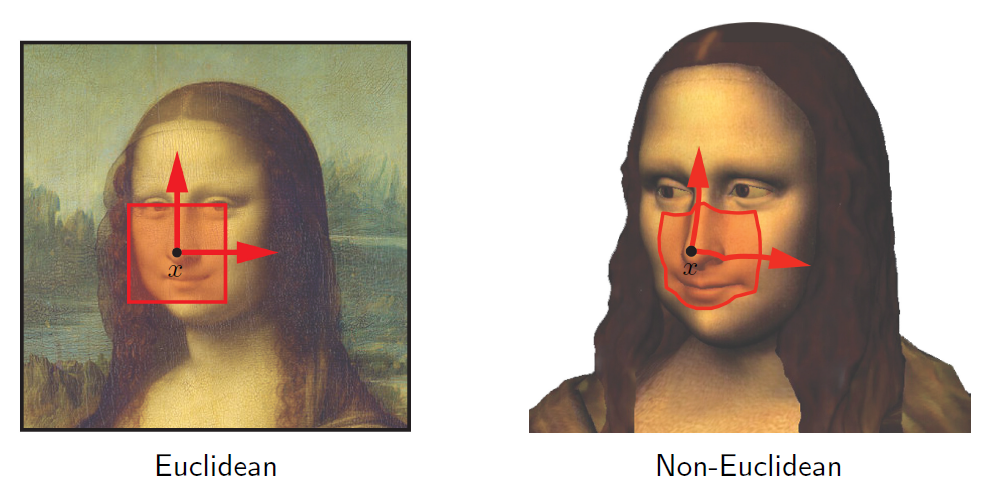
\includegraphics[width=.7\textwidth]{figures/12/monalisa-conv.png}
    \caption{Idea of convolution on a mesh.}
\end{figure}

\begin{figure}[H]
    \centering
    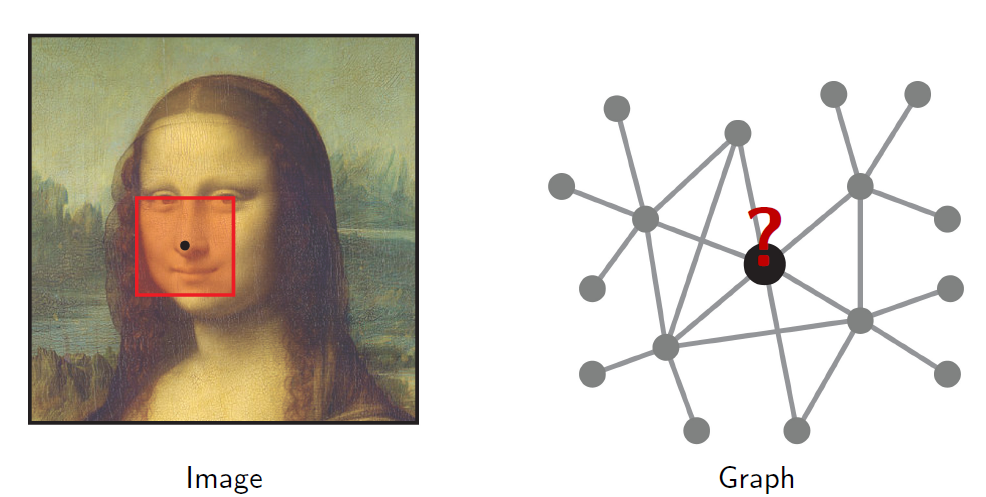
\includegraphics[width=.7\textwidth]{figures/12/monalisa-graph.png}
    \caption{Not really clear how to define non-Euclidean convolution on graphs...}
\end{figure}